\documentclass[compress,xcolor=table]{beamer}
% add handout to optional args for handout version

\usepackage{beamerthemesplit}
\usepackage[utf8]{inputenc}
\usepackage[german]{babel}
\usepackage{german}
\usepackage{graphicx}
\usepackage{subfigure}
\usepackage{wrapfig}
\usepackage{epsfig}
\usepackage{tabularx}
\usepackage{latexsym}
\usepackage{url}
\usepackage{tikz}
\usepackage{multimedia}
\usepackage{xcolor}
\usepackage{eso-pic}
\usepackage{color}
\usepackage{type1cm}
\usepackage{listings}
\usepackage{verbatim}
\usepackage{colortbl}
\usepackage{psfrag}
\usepackage{xifthen}
\usepackage[absolute,overlay]{textpos}
\usepackage{palatino}
\usepackage{appendixnumberbeamer}

%% Mulberry Color for highlighting
\definecolor{Mulberry}{cmyk}{0.34,0.90,0,0.02}
\definecolor{Lavender}{cmyk}{0,0.48,0,0}
\definecolor{Melon}{cmyk}{0,0.46,0.50,0}
\definecolor{Peach}{cmyk}{0,0.50,0.70,0}
\definecolor{RedOrange}{cmyk}{0,0.77,0.87,0}
\definecolor{BrickRed}{cmyk}{0,0.89,0.94,0.28}
\definecolor{Mahogany}{cmyk}{0,0.85,0.87,0.35}
\definecolor{BurntOrange}{cmyk}{0,0.51,1,0}
\definecolor{BitterSweet}{cmyk}{0,0.75,1,0.24}
\definecolor{FawkesRed}{rgb}{0.53,0,0}
\definecolor{RosBlue}{rgb}{0.19,0.25,0.38}


\mode<presentation>
{
  \usetheme{FawkesSimple}

  % to hide nav bar uncomment this line
  \setbeamertemplate{navigation symbols}{}

  %\setbeamercovered{transparent}
  \setbeamercovered{%
    again covered={\opaqueness<1->{40}}
  }
}

% Usage notes for handout version:
% Compile the beamer version immediately before you build the handout version,
% otherwise page numbers etc. will be wrong! The .aux files are *not* updated
% in handout mode, see PGF Manual for details why this is necessary.
% Comment out below one of the two pgfuselayout lines for either 2 or 4 slides
% per page. To have a very light grey background uncomment the background canvas
% color line. The logical page options are used to draw borders around each
% slide.
\mode<handout>
{
  \usetheme{FawkesSimple}

  % to hide nav bar uncomment this line
  \setbeamertemplate{navigation symbols}{}

  %\setbeamercovered{transparent}
  \setbeamercovered{%
    again covered={\opaqueness<1->{40}}
  }

  % Very slight grey background, can be used instead of borders
  %\setbeamercolor{background canvas}{bg=black!5}

  \usepackage{pgfpages}
  %% \pgfpagesuselayout{4 on 1}[a4paper,border shrink=5mm,landscape]
  \pgfpagesuselayout{2 on 1}[a4paper,border shrink=5mm]

  \pgfpageslogicalpageoptions{1}{border code=\pgfstroke}
  \pgfpageslogicalpageoptions{2}{border code=\pgfstroke}
  \pgfpageslogicalpageoptions{3}{border code=\pgfstroke}
  \pgfpageslogicalpageoptions{4}{border code=\pgfstroke}
  \nofiles
}


% Declare layers
\pgfdeclarelayer{background}
\pgfsetlayers{background,main} 

% Load PGF libraries
\usetikzlibrary{patterns}
\usetikzlibrary{arrows}
\usetikzlibrary{topaths}
\usetikzlibrary{snakes}
\usetikzlibrary{calc}
\usetikzlibrary{positioning}
\usetikzlibrary{shadows}
\usetikzlibrary{shapes.multipart}


% set lengths for textpos package
\setlength{\TPHorizModule}{10mm}
\setlength{\TPVertModule}{\TPHorizModule}
\textblockorigin{8mm}{16mm} % start everything near the top-left corner
\setbeamercolor{textblock color}{fg=blue!50,bg=white}

\urlstyle{sf}
\urldef{\projecturl}\url{}

%\pgfdeclareimage[width=4cm]{logo-big}{syslife/logo_big}

\institute{%
  %\vspace{1cm}
  \begin{minipage}{\textwidth}\centering
  
\includegraphics[height=0.6cm]{images/rwth-logo}
  \end{minipage}

  \bigskip

  \begin{minipage}{\textwidth}\centering
  \textcolor{FawkesBrown}
  \projecturl
  \end{minipage}
  %\vspace{-1.5cm}
    %  \end{column}
    %\end{columns}
  %\end{minipage}
}


%\titlegraphic{\pgfuseimage{logo-big}}

% \AtBeginPart{\frame{\partpage}}

%numbers=left, numberstyle=\tiny, stepnumber=2, numbersep=5pt
\lstset{language=[GNU]C++,
        basicstyle=\small,
        escapeinside={/*(*/}{/*)*/},
        breaklines=true,
        showstringspaces=false
        }

\lstdefinelanguage{JavaScript}{
  keywords={typeof, new, true, false, catch, function, return, null, catch, switch, var, if, in, while, do, else, case, break},
  keywordstyle=\color{blue}\bfseries,
  ndkeywords={class, export, boolean, throw, implements, import}, %, this
  ndkeywordstyle=\color{darkgray}\bfseries,
  identifierstyle=\color{black},
  sensitive=false,
  comment=[l]{//},
  morecomment=[s]{/*}{*/},
  commentstyle=\color{purple}\ttfamily,
  stringstyle=\color{red}\ttfamily,
  morestring=[b]',
  morestring=[b]"
}

\lstdefinestyle{JSON}
{
  language=JavaScript,
  morekeywords={interface,field,message,comment},
  basicstyle=\footnotesize\ttfamily\vspace{0.2cm},
  breaklines=true,
  showstringspaces=false,
  %keywordstyle=\bfseries,
  keywordstyle=\color{Mulberry},
  frame=lines,
  belowcaptionskip=8pt,
  emphstyle=\itshape,
  numbers=left,
  stepnumber=1,
  backgroundcolor=\color{blue!10},
  rulecolor=\color{blue!50},
  fillcolor=\color{blue!20},
  framexleftmargin=16pt,
  xleftmargin=16pt,
  %stringstyle=\color{BitterSweet},
  stringstyle=\color{BrickRed},
  commentstyle=\color{BrickRed},
  escapechar=\%
  % emph={getup, servo, depends_skills},
  %emphstyle=\underbar,
  %numbers=left,
  %stepnumber=1,
  %%stringstyle=\ttfamily, % typewriter type for strings
}

\lstdefinestyle{SmallJSON}{
  style=JSON,
  basicstyle=\ttfamily\footnotesize,
  numbersep=6pt,
}
\lstdefinestyle{ReallySmallJSON}{
  style=JSON,
  basicstyle=\ttfamily\tiny,
  numbersep=5pt,
}


% Listings stuff
\lstdefinelanguage{Lua}
{
  morekeywords={and,break,do,else,elseif,end,false,for,function,
                if,in,local,nil,not,or,repeat,return,then,true,until,while},
  sensitive=true,
  morecomment=[l]{--},
  morecomment=[s]{--[[}{--]]},
  morestring=[b]{"},
  morestring=[s]{[==[}{]==]},
}

% default style
\lstdefinestyle{Lua}
{
  language=Lua,
  basicstyle=\ttfamily,
  breaklines=true,
  showstringspaces=false,
  %keywordstyle=\bfseries,
  keywordstyle=\color{Mulberry},
  %frame=lines,
  %belowcaptionskip=8pt,
  emphstyle=\itshape,
  %numbers=left,
  stepnumber=1,
  %backgroundcolor=\color{blue!10},
  rulecolor=\color{blue!50},
  fillcolor=\color{blue!20},
  %framexleftmargin=18pt,
  %xleftmargin=18pt,
  stringstyle=\color{BitterSweet},
  %stringstyle=\color{BrickRed},
  commentstyle=\color{BrickRed},
  escapechar=\%
  % emph={getup, servo, depends_skills},
  %emphstyle=\underbar,
  %numbers=left,
  %stepnumber=1,
  %%stringstyle=\ttfamily, % typewriter type for strings
}
\lstdefinestyle{SmallLua}{
  style=Lua,
  basicstyle=\ttfamily\footnotesize,
  numbersep=6pt,
}
\lstdefinestyle{ReallySmallLua}{
  style=Lua,
  basicstyle=\ttfamily\tiny,
  numbersep=5pt,
}

% Default is Lua
\lstset{style=Lua}


% Hyphenation of words with hyphen
\def\hyph{-\penalty0\hskip0pt\relax}


% define an anchor in the frame
\newcommand{\tikzref}[1]{%
  \tikz[remember picture]{%
    \coordinate (#1) at (0,0.5ex);%
  }%
}%


%%% Local Variables: 
%%% mode: latex
%%% TeX-master: "iros2012-robodb"
%%% End: 


\newcommand{\backupbegin}{
   \newcounter{finalframe}
   \setcounter{finalframe}{\value{framenumber}}
}
\newcommand{\backupend}{
   \setcounter{framenumber}{\value{finalframe}}
}

% define vector/matrix helpers
\newcommand*\colvec[3][]{
    \begin{pmatrix}\ifx\relax#1\relax\else#1\\\fi#2\\#3\end{pmatrix}
}
\newcommand{\mattwo}[4]{\begin{pmatrix} #1 & #2 \\ #3 & #4\end{pmatrix}}


\title[Combining 3D Shape, Color, and Motion for Robust Anytime Tracking]{Combining 3D Shape, Color, and Motion\\ for Robust Anytime Tracking\\ \small{Paper by Held, Levinson, Thrun, and Savarese~\cite{paper}}}
\author[Zwilling]{%
  Frederik Zwilling\\
  \bigskip
  {\scriptsize Seminar Current Topics in Computer Vision and Machine Learning\\ RWTH Aachen University}
}

\date[\today @ Seminar CVML]{\today -- Seminar Current Topics in Computer Vision and Machine Learning}

\begin{document}

\frame[plain]{\titlepage}
\addtocounter{framenumber}{-1}

\begin{frame}
  \frametitle{Agenda}
  \tableofcontents[hideallsubsections]
\end{frame}

\section{Motivation}

\begin{frame}
  \frametitle{Tracking for Autonomous Cars}
  
  \begin{columns}
  \begin{column}{0.6\textwidth}
  \begin{description}[]
  \item[Chances] \hfill \\
  \begin{itemize}
  \item Free use of driving time
  \item Help disabled persons
  \item Computers do not get\\tired or drunk
  \item Faster reaction time
  \item[$\Rightarrow$] Safe 26k lives per year in EU
  \end{itemize}
  \end{description}
  \end{column}
  \begin{column}{0.4\textwidth}
  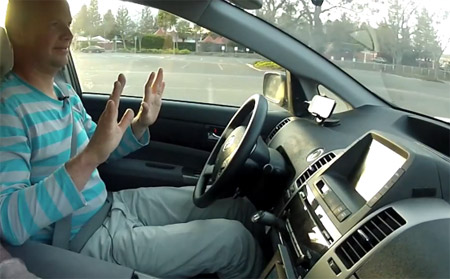
\includegraphics[width=\textwidth]{images/auto.jpg}
  \end{column}
  \end{columns}
  \pause
  \bigskip
  \begin{columns}
  \begin{column}{0.6\textwidth}
  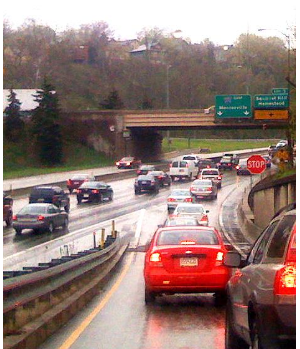
\includegraphics[height=0.35\textheight]{images/highway}
  \hspace{0.01cm}
  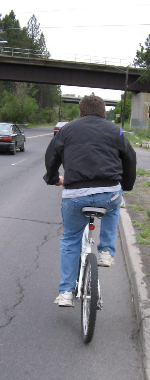
\includegraphics[height=0.35\textheight]{images/cycle}
  \hspace{0.01cm}
  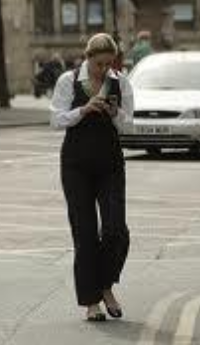
\includegraphics[height=0.35\textheight]{images/pedestrian}
  \end{column}
  \begin{column}{0.5\textwidth}
  \begin{description}[]
  \item[Challenges] \hfill \\
  \begin{itemize}
  \item Precise tracking
  \item Robustness
  \item Occlusion
  \item Real time
  \end{itemize}
  \end{description}
  \end{column}
  \end{columns}
\end{frame}

\begin{frame}
  \frametitle{Tracking for Autonomous Cars}
  \begin{description}[]
  \item[Subtasks of Tracking] \hfill \\
  \begin{itemize}
  \item Segment sensor data into objects
  \item Associate objects in successive frames
  \item Position and velocity estimation
  \item Object and trajectory classification
  \end{itemize}
  \end{description}
  \pause
  \begin{block}{Topic of this presentation}
    Position and velocity estimation
  \end{block}
\end{frame}

\begin{frame}
  \frametitle{Given Sensor Data}

  \begin{columns}
  \begin{column}{0.6\textwidth}
  \begin{description}[]
  \item[Sensor] \hfill \\
  \begin{itemize}
  \item Dense 3D laser sensor
  \item Generates point cloud
  \item Additional panorama image
  \item Similar to stereo cameras\\
        but more precise and expensive
  \end{itemize}
  \pause
  \item[Given for us] \hfill \\
  \begin{itemize}
  \item Point clouds of detected objects
  \item Association between frames already done
  \end{itemize}
  \end{description}
  \end{column}
  \onslide<1->
  \begin{column}{0.4\textwidth}
%%   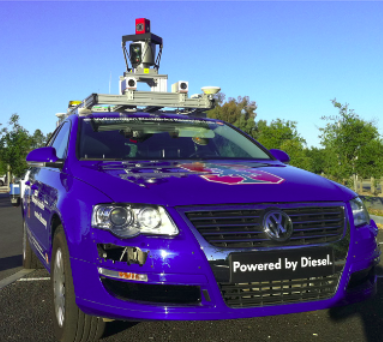
\includegraphics[width=\textwidth]{../img/lidar}\\
%% \bigskip
%%   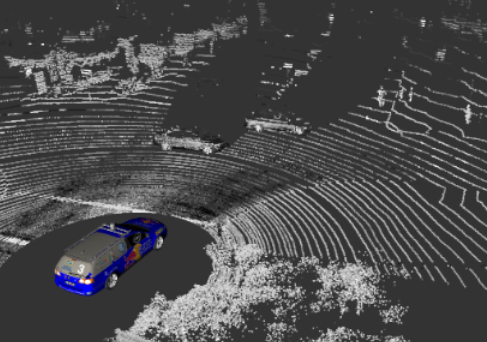
\includegraphics[width=\textwidth]{../img/lidar-data}

  \begin{tikzpicture}[thick, every node/.style={font=\footnotesize}]
    \node (program) [outer sep=0,inner sep=0,anchor=south west]
    at (0,0)
    {
    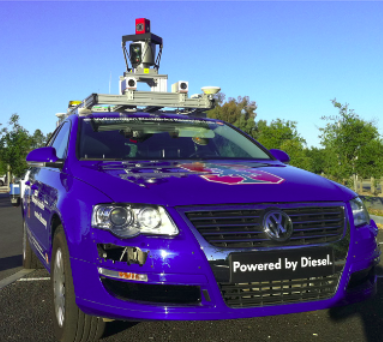
\includegraphics[width=\textwidth]{../img/lidar}};
    \node (program) [outer sep=0,inner sep=0,anchor=south west]
    at (0,-3.3)
    {
    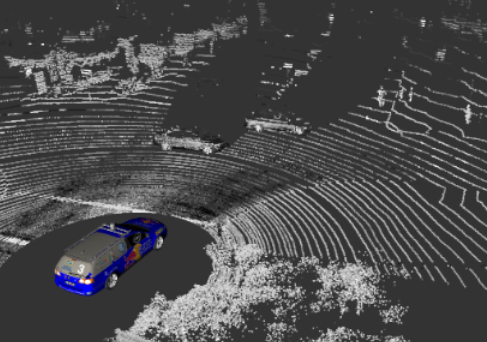
\includegraphics[width=\textwidth]{../img/lidar-data}};
    \node (descx) at (4.7,-3.4)
    {\tiny \cite{arbitrary-object-recognition}};
    \onslide<1->
  \end{tikzpicture}  
  \end{column}
  \end{columns}
\end{frame}

\begin{frame}
  \frametitle{Teaser Paper Ideas}
  \begin{description}[]
  \item[How to find a precise alignment?] \hfill \\
  \begin{itemize}
  \item Utilize whole object shape
  \item Additional cues from color
  \item Use motion model
  \end{itemize}
  \pause
  \item[How to search the state space fast?] \hfill \\
  \begin{itemize}
  \item Histogram with coarse initial resolution
  \item Refine resolution important areas
  \item Consider resolution in the probabilistic model
  \end{itemize}
  \end{description}
\end{frame}


\section{Baseline Methods}
\begin{frame}
  \frametitle{Baseline Methods}
  \begin{tikzpicture}[thick, every node/.style={font=\footnotesize}]
    \only<1>{
    \node (program) [outer sep=0,inner sep=0,anchor=south west]
    at (0,0)
    {
    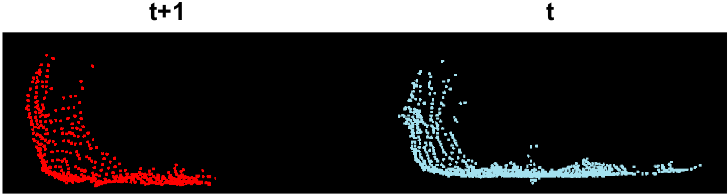
\includegraphics[width=\textwidth,height=0.25\textwidth]{images/point-clouds}};}
    \only<2>{
    \node (program) [outer sep=0,inner sep=0,anchor=south west]
    at (0,0)
    {
    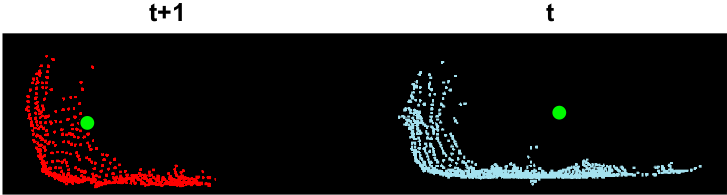
\includegraphics[width=\textwidth,height=0.25\textwidth]{images/centroid}};}
    \only<3>{
    \node (program) [outer sep=0,inner sep=0,anchor=south west]
    at (0,0)
    {
    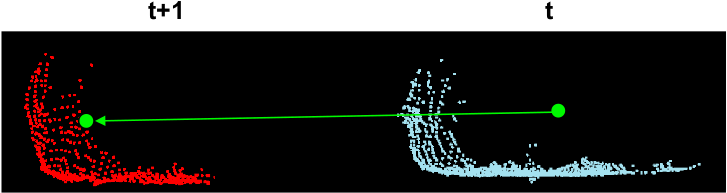
\includegraphics[width=\textwidth,height=0.25\textwidth]{images/centroid-alignment}};}
    \only<4->{
    \node (program) [outer sep=0,inner sep=0,anchor=south west]
    at (0,0)
    {
    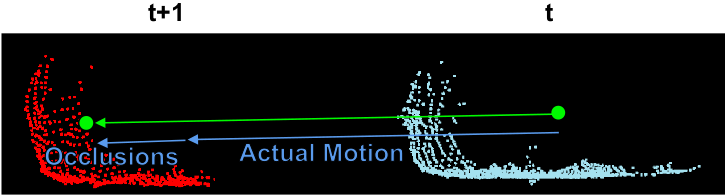
\includegraphics[width=\textwidth,height=0.25\textwidth]{images/kalman-error}};}
    \node (descx) at (10.6,-0.25)
    {\tiny \cite{held-website}};
    \onslide<1->
  \end{tikzpicture}
  
  \begin{description}[]
  \item[Kalman Filter] \hfill \\
  \begin{itemize}
  \onslide<2->{\item Aligns centroids}
  \onslide<4->{\item Problems with occlusion}
  \onslide<5->{\item Robustness through motion model}
  \onslide<6->{\item Very fast}
  \end{itemize}
  \end{description}
\end{frame}

\begin{frame}
  \frametitle{Baseline Methods}
  
  \begin{description}[]
  \item[Iterative Closest Point (ICP)] \hfill \\
  \begin{itemize}
  \item Iterative hill climbing approach
  \item Minimizes quadratic distance of closest points
  \item Uses whole point cloud
  \pause
  \item Depends on good initialization
  \item Problem: local optima\\
  \begin{tikzpicture}[thick, every node/.style={font=\footnotesize}]
    \only<1-2>{
    \node (program) [outer sep=0,inner sep=0,anchor=south west]
    at (0,0)
    {
    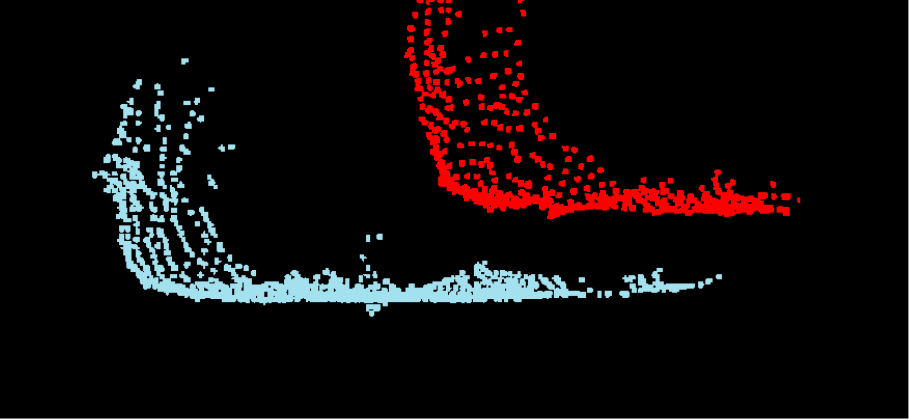
\includegraphics[height=0.25\textwidth]{images/icp-init}};}
    \only<3>{
    \node (program) [outer sep=0,inner sep=0,anchor=south west]
    at (0,0)
    {
    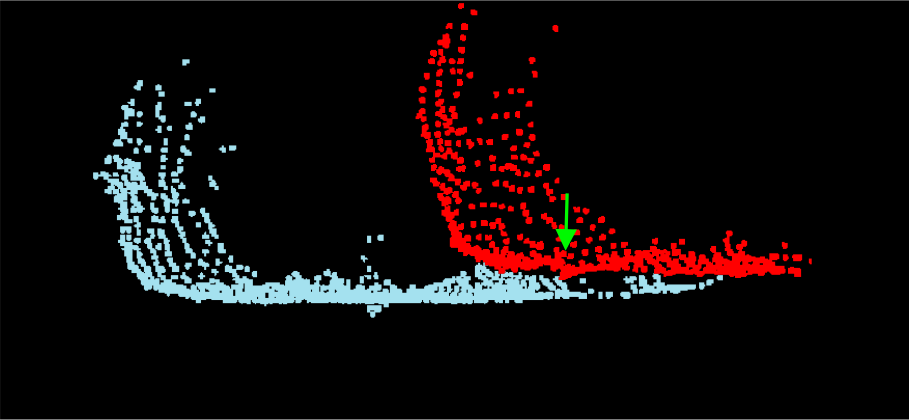
\includegraphics[height=0.25\textwidth]{images/icp-1}};}
    \only<4>{
    \node (program) [outer sep=0,inner sep=0,anchor=south west]
    at (0,0)
    {
    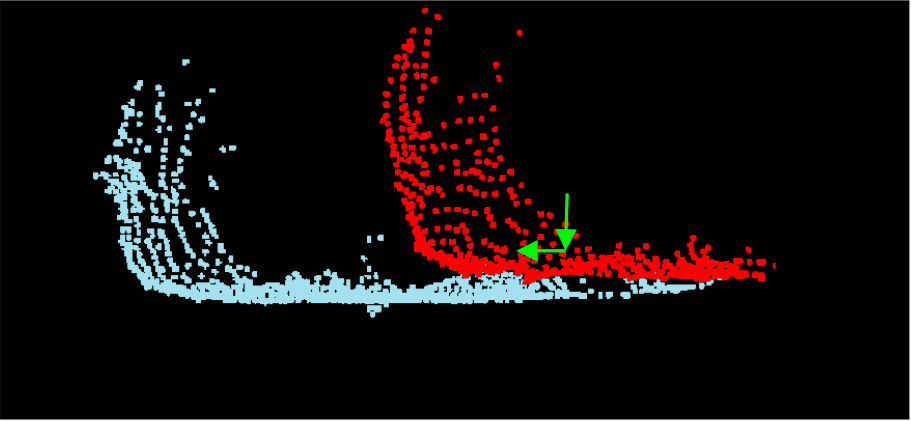
\includegraphics[height=0.25\textwidth]{images/icp-2}};}
    \only<5->{
    \node (program) [outer sep=0,inner sep=0,anchor=south west]
    at (0,0)
    {
    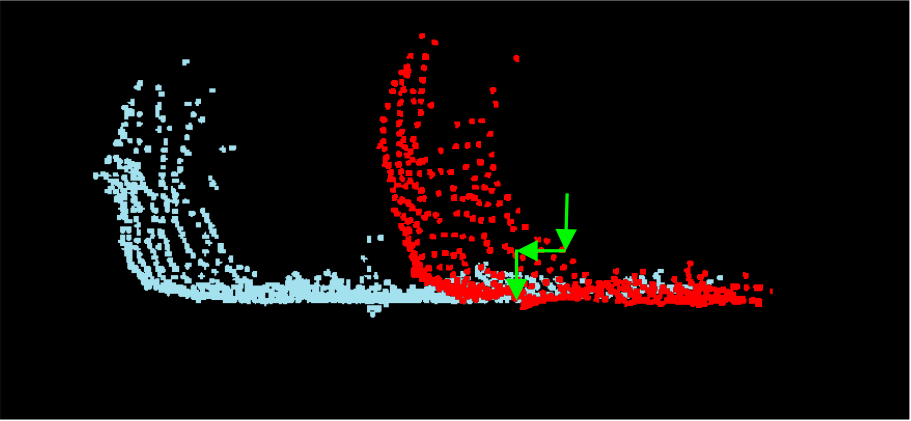
\includegraphics[height=0.25\textwidth]{images/icp-3}};}
    \node (descx) at (5.7,-0.2)
    {\tiny \cite{held-website}};
    \onslide<1->
  \end{tikzpicture}
  \pause
  \pause
  \pause
  \item No motion model
  \end{itemize}
  \end{description}
\end{frame}


\section{Probabilistic Model}

\begin{frame}
  \frametitle{Probabilistic Model}      
  \center
  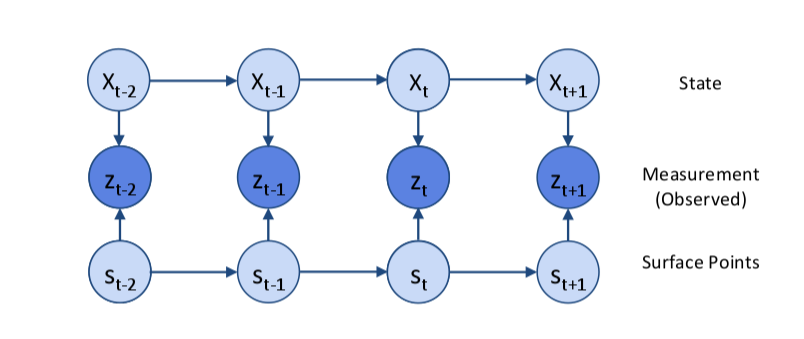
\includegraphics[width=0.8\textwidth]{../img/dbn}
  {\tiny \cite{paper}}
  \begin{description}[]
  \item[Dynamic Bayesian Network] \hfill \\
  \begin{itemize}
  \item Relates variables over successive frames
  \item State $x_t$ (position relative to last frame and velocity)\\
        Surface points $s_t=\{s_{t,1},...,s_{t,n}\}$\\
        Measured point cloud $z_t=\{z_{t,1},...,z_{t,n}\}$
  \item Rotation not considered
  \end{itemize}
  \end{description}
\end{frame}

\begin{frame}
  \frametitle{Probabilistic Model}
  \begin{columns}
  \begin{column}{0.62\textwidth}
  \begin{description}[]
  \item[Surface points] \hfill \\
  \begin{itemize}
  \item Sampled from the visible surface
  \item Indirectly observable
  \item Visible surface varies due to occlusion and viewpoint changes
  \item $p(s_{t,i}|s_{t-1})=p(V)*p(s_{t,i}|s_{t-1},V)+$\\$p(\neg V)*p(s_{t,i}|s_{t-1},\neg V)$
  \item[$\Rightarrow$] $p(s_{t}|s_{t-1}) = \eta(\mathcal{N}(s_t;s_{t-1,i},\Sigma_r) + k)$
  \end{itemize}
  \end{description}
  \end{column}
  \begin{column}{0.4\textwidth}
  \begin{tikzpicture}[thick, every node/.style={font=\footnotesize}]
    \node (program) [outer sep=0,inner sep=0,anchor=south west]
    at (0,0)
    {
    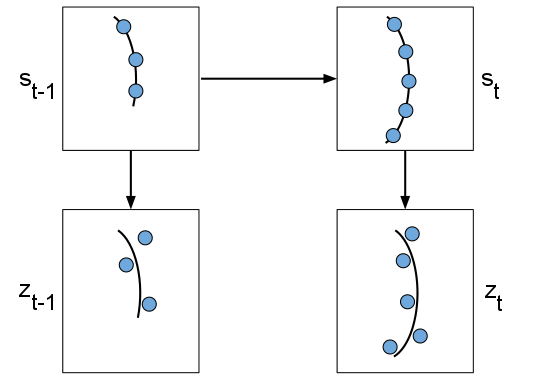
\includegraphics[width=\textwidth]{../img/surface-measurement}};
    \node (descx) at (4.3,-0.2)
    {\tiny \cite{paper}};
  \end{tikzpicture}
  \end{column}
  \end{columns}
\end{frame}

\begin{frame}
  \frametitle{Probabilistic Model}
  \begin{columns}
  \begin{column}{0.62\textwidth}
  \begin{description}[]
  \item[Measurement points] \hfill \\
  \begin{itemize}
  \item Depending on surface points
  \item Gaussian sensor noise $\Sigma_e$
  \item $z_{t,i} \sim \mathcal{N}(s_{t,i},\Sigma_e) + x_{t,p}$\\
        $z_{t-1,i} \sim \mathcal{N}(s_{t-1,i},\Sigma_e)$
  \end{itemize}
  \end{description}
  \end{column}
  \begin{column}{0.4\textwidth}
  \begin{tikzpicture}[thick, every node/.style={font=\footnotesize}]
    \node (program) [outer sep=0,inner sep=0,anchor=south west]
    at (0,0)
    {
    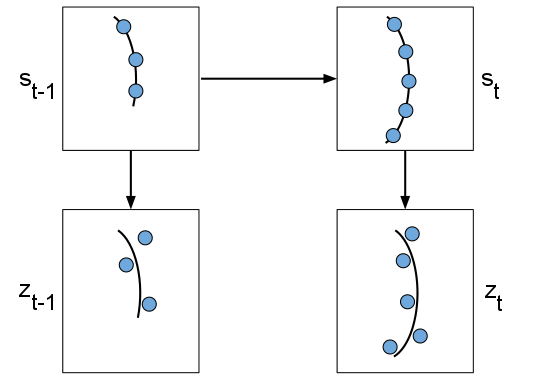
\includegraphics[width=\textwidth]{../img/surface-measurement}};
    \node (descx) at (4.3,-0.2)
    {\tiny \cite{paper}};
  \end{tikzpicture}
  \end{column}
  \end{columns}
\end{frame}

\begin{frame}
  \frametitle{Probabilistic Model}

  \begin{columns}
  \begin{column}{0.4\textwidth}
  \begin{description}[]
  \item[Measurement Model] \hfill \\
  \end{description}
  \end{column}
  \begin{column}{0.6\textwidth}
  \vspace{1cm}
  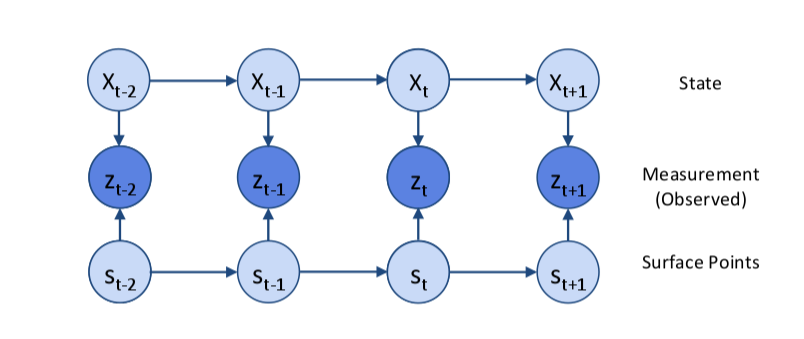
\includegraphics[width=0.9\textwidth]{../img/dbn}
  \end{column}
  \end{columns}
  \vspace{-1cm}
  \begin{align}     
    p(z_t|x_t,z_1,...,z_{t-1}) \onslide<2-> & \approx p(z_t|x_t,z_{t-1}) \nonumber\\
    \onslide<3-> &= \int \int p(z_t,s_t,s_{t-1}|x_t,z_{t-1}) \mathrm d s_t \mathrm d s_{t-1} \nonumber\\
    \onslide<4-> &= \underbrace{\int p(z_t|s_t,x_t) \underbrace{\int p(s_t|s_{t-1})\eta p(z_{t-1}|s_{t-1}) \mathrm d s_t}_{\text{convolution}} \mathrm d s_{t-1}}_{\text{convolution}} \nonumber\\
    \onslide<5-> &= \eta(\mathcal{N}(z_t;z_{t-1}+x_{t,p},\Sigma_r+2\Sigma_e)+k) \nonumber
    \onslide<1->
  \end{align}
\end{frame}

\newcommand{\unaryminus}{\scalebox{0.75}[1.0]{\( - \)}}

\begin{frame}
  \frametitle{Probabilistic Model}
  \begin{description}[]
  \item[Measurement Model Computation] \hfill \\
  \begin{itemize}
  \item $ccp(z_{t,i})$: closest correspondence point in $z_{t-1}+x_{t,p}$
  \pause
  \item Covariance matrix $\Sigma = 2\Sigma_e+\Sigma_r$
  %say: sigma r funciton of distance
  \pause
  \item Normalization constant $\eta$
  \item Smoothing factor $k$
  %say: found by training
  \onslide<1->
  \end{itemize}
  \end{description}     
  \begin{block}{Measurement Probability}
  \small
  $$
  p(z_t|x_t,z_{t-1}) =
  \eta\prod\limits_{z_{t,i}\in z_t}
  \mathrm{exp}\left(\unaryminus\frac{1}{2}(z_{t,i}\unaryminus\mathrm{ccp}(z_{t,i}))^T\Sigma^{\unaryminus 1}(z_{t,i}\unaryminus\mathrm{ccp}(z_{t,i}))\right)+k
  \nonumber
  $$
  \end{block}
\end{frame}

\begin{frame}
  \frametitle{Probabilistic Model}
  \begin{itemize}
  \item Align smaller point cloud in larger one\\
  \only<1>{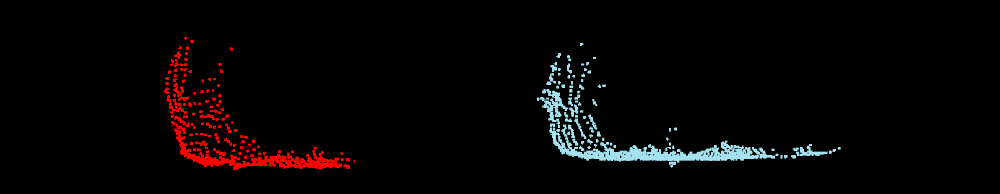
\includegraphics[width=0.9\textwidth]{images/align-init}}
  \only<2->{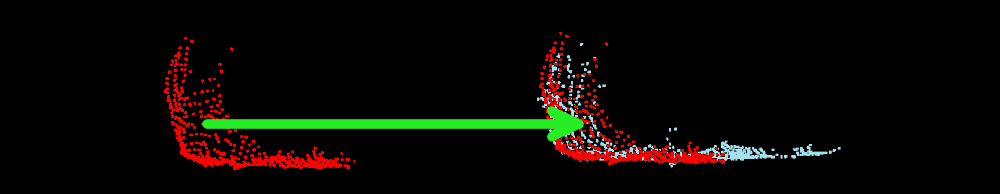
\includegraphics[width=0.9\textwidth]{images/align-small}}
  \pause
  \pause
  \item Aligning larger point cloud in smaller one\\
  \only<3>{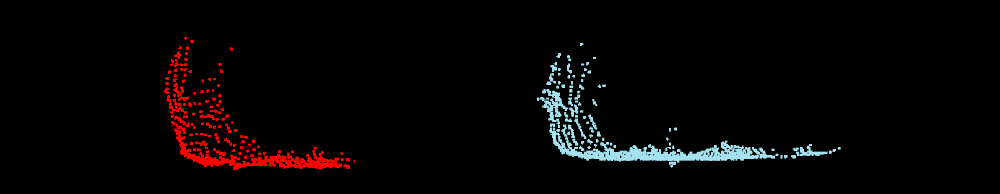
\includegraphics[width=0.9\textwidth]{images/align-init}}
  \onslide<4->{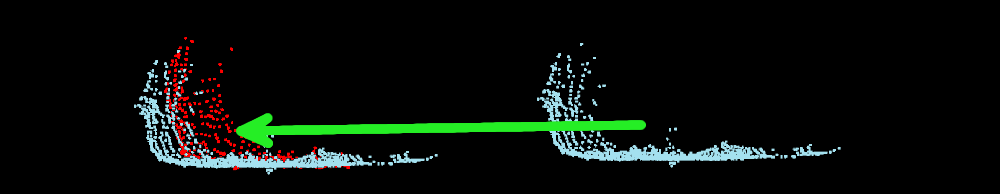
\includegraphics[width=0.9\textwidth]{images/align-larger}}
  \pause
  \pause
  \item[$\Rightarrow$] Exchange $z_t$ and $z_{t-1}$ when $|z_t|>|z_{t-1}|$
  \end{itemize}
\end{frame}

\begin{frame}
  \frametitle{Probabilistic Model}
  \begin{description}[]
  \item[Adding Color] \hfill \\
  \begin{itemize}
  \item Use available color information of measurement points
  \item Better alignment despite occlusions
  \item Embed color matching into measurement model
  \begin{align}
p_c(s_{t,i}|s_{t-1},V)
  = &p(C)p_c(s_{t,i}|s_{t-1},V,C)+ \nonumber\\
&p(\neg C)p_c(s_{t,i}|s_{t-1},V,\neg C)\nonumber
  \end{align}
  \begin{itemize}
  \item $p(C)$: Color-model applicable
  \item $p(\neg C)$: Color-model not applicable (lens flare, reflections)
  \item $p_c(s_{t,i}|s_{t-1},V,\neg C)=\frac{1}{255}$: Color mismatch
  \item $p_c(s_{t,i}|s_{t-1},V,C)$: Color match
  \end{itemize}
  \end{itemize}
  \end{description}
\end{frame}

\begin{frame}
  \frametitle{Probabilistic Model}
  \begin{description}[]
  \item[Motion Model] \hfill \\
  \begin{itemize}
  \item Take whole measurement history into account
  \item Robustness against single imprecise alignments
  \pause
  \item Kalman filter with constant velocity model
  \item Measurement step: update with Gaussian distribution\\
        $\mu_t=\sum_i p(x_{t,i}|z_1,...,z_t)x_{t,i}$\\
        $\Sigma_t=\sum_i p(x_{t,i}|z_1,...,z_t) (x_{t,i}-\mu_t)(x_{t,i}-\mu_t)^T$
  \item Update step: apply velocity to position
  \end{itemize}
  \end{description}
\end{frame}


\section{Searching the State Space}
\begin{frame}
  \frametitle{Searching the State Space}
  \begin{description}[]
  \item[Search the State Space] \hfill \\
  \pause
  \begin{itemize}
  \item For most likely state
  \item Globally, without getting stuck in local optima
  \item Allow multiple hypotheses
  \pause
  \item[$\Rightarrow$] Use histogram
  \pause
  \item[$\Rightarrow$] Too slow for necessary resolution
  \end{itemize}
  \end{description}
  \onslide<3->
  \begin{tikzpicture}[thick, every node/.style={font=\footnotesize}]
    \node (program) [outer sep=0,inner sep=0,anchor=south west]
    at (0,0)
    {
    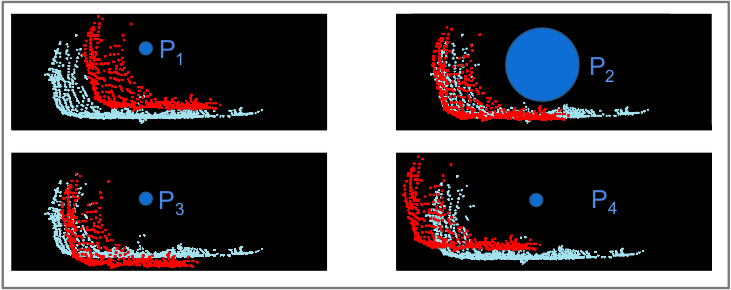
\includegraphics[width=\textwidth]{images/histogram}};
    \node (descx) at (11,-0.2)
    {\tiny \cite{held-website}};
  \end{tikzpicture}
\end{frame}

\begin{frame}
  \frametitle{Searching the State Space}
  \begin{description}[]
  \item[In Real Time] \hfill \\
  \begin{itemize}
  \item Densely sample only areas with high probability
  \item Initial coarse resolution
  \item Stop at anytime during refinement
  \pause
  \item[$\Rightarrow$] Use dynamic histogram
  \end{itemize}
  \end{description}
  \onslide<1->
  \begin{tikzpicture}[thick, every node/.style={font=\footnotesize}]
    \node (program) [outer sep=0,inner sep=0,anchor=south west]
    at (0,0)
    {
    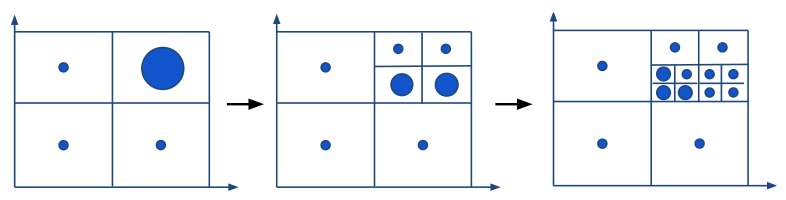
\includegraphics[width=\textwidth]{images/adh}};
    \node (descx) at (11,-0.2)
    {\tiny \cite{paper}};
  \end{tikzpicture}
\end{frame}

\begin{frame}
  \frametitle{Searching the State Space}
  \begin{description}[]
  \item[Derivation Step] \hfill \\
  \begin{itemize}
  \item Recursively expend cells\\
  \begin{tikzpicture}[thick, every node/.style={font=\footnotesize}]
    \node (program) [outer sep=0,inner sep=0,anchor=south west]
    at (0,0)
    {
    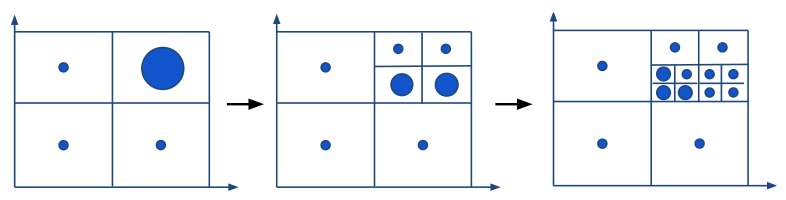
\includegraphics[width=0.5\textwidth]{images/adh}};
    \node (descx) at (5.5,0)
    {\tiny \cite{paper}};
  \end{tikzpicture}
  \pause
  \item Maximize information gain / Minimize KL-divergence\\
  \begin{tikzpicture}[thick, every node/.style={font=\footnotesize}]
    \node (program) [outer sep=0,inner sep=0,anchor=south west]
    at (0,0)
    {
    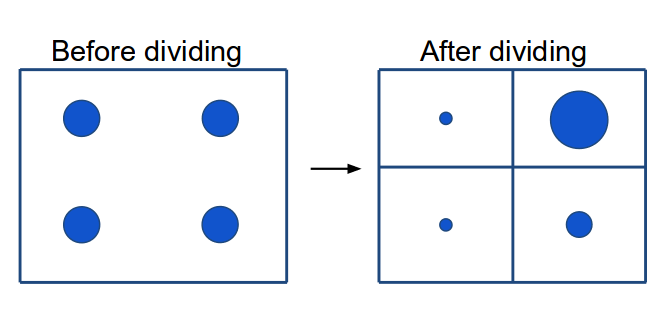
\includegraphics[width=0.4\textwidth]{../img/devision-criteria}};
    \node (descx) at (4.3,0)
    {\tiny \cite{paper}};
  \end{tikzpicture}
  \pause
  \item KL-divergence: information loss if A approximated by B
  $$D_{KL}(A||B)=\sum_{j=1}^k p_j \mathrm{ln}\left(\frac{p_j}{P_i/k}\right)$$
  \end{itemize}
  \end{description}
\end{frame}

\begin{frame}
  \frametitle{Searching the State Space}
  \begin{description}[]
  \item[Annealing Dynamic Histogram (ADH)] \hfill \\
  \begin{itemize}
  \item No good alignment with coarse resolution
  \item Sampling resolution another error source
  \item[$\Rightarrow$] Consider sampling resolution in measurement model
  \item $\Sigma = 2\Sigma_e+\Sigma_r+\Sigma_g$
  \item $\Sigma_g$ proportional to sampling resolution
  \end{itemize}
  \end{description}
\end{frame}

\section{Evaluation}
\begin{frame}
  \frametitle{Evaluation}
  \begin{description}[]
  \item[What to evaluate] \hfill \\
  \begin{itemize}
  \item Precision of the position and velocity estimation
  \item Root-Mean-Square error
        $$e_{RMS}=\sqrt{\mathbb{E}((\hat{v}_t-v_t)^2)}$$
  \item Runtime (real time requirements)
  \item Comparison to baseline methods
  \item[$\Rightarrow$] Need for test data
  \end{itemize}
  \end{description}
\end{frame}

\begin{frame}
  \frametitle{Evaluation}
  \begin{columns}
  \begin{column}{0.6\textwidth}
  \begin{description}[]
  \item[Relative Reference Frame Approach] \hfill \\
  \begin{itemize}
  \item Record sensor data while driving
  \item Static environment
  \item Assume car is standing still
  \pause
  \item Compute ground truth position and velocity\\ from distance and car velocity
  \onslide<1->
  \end{itemize}
  \end{description}
  \end{column}
  \begin{column}{0.4\textwidth}
  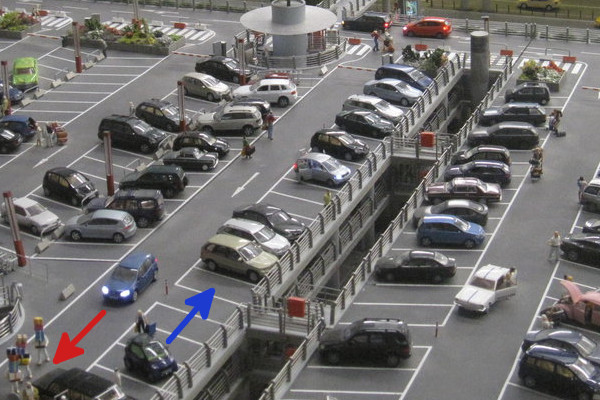
\includegraphics[width=\textwidth]{images/parking}\\
  \begin{tikzpicture}[thick, every node/.style={font=\footnotesize}]
    \node (program) [outer sep=0,inner sep=0,anchor=south west]
    at (0,0)
    {
      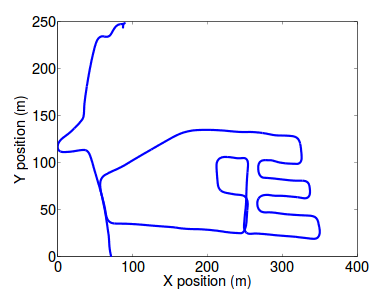
\includegraphics[width=\textwidth]{images/rel-ref-frame-path}};
      \node (descx) at (4.5,-0.2){\tiny \cite{paper}};
  \end{tikzpicture}
  \end{column}
  \end{columns}
\end{frame}

\begin{frame}
  \frametitle{Evaluation}
  \begin{columns}
  \begin{column}{0.6\textwidth}
  \begin{description}[]
  \item[Kalman Filter] \hfill \\
  \begin{itemize}
  \item Imprecise but very fast
  \end{itemize}
  \pause
  \item[ICP] \hfill \\
  \begin{itemize}
  \item Slow and very imprecise
  \item Variants with motion model perform better
  \end{itemize}
  \pause
  \item[ADH] \hfill \\
  \begin{itemize}
  \item Quick first result
  \item Outperforms all baseline methods
  \end{itemize}
  \onslide<1->
  \end{description}
  \end{column}
  \begin{column}{0.5\textwidth}
  \begin{tikzpicture}[thick, every node/.style={font=\footnotesize}]
    \node (program) [outer sep=0,inner sep=0,anchor=south west]
    at (0,0)
    {
    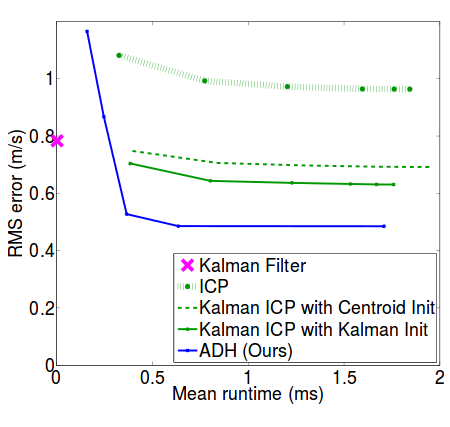
\includegraphics[width=\textwidth]{../img/rms-vs-runtime}};
    \node (descx) at (5.5,-0.2)
    {\tiny \cite{paper}};
  \end{tikzpicture}
  \end{column}
  \end{columns}
\end{frame}

\begin{frame}
  \frametitle{Evaluation}
  \begin{description}[]
  \item[ADH acceleration] \hfill \\
  \begin{itemize}
  \item[] 
  \begin{tikzpicture}[thick, every node/.style={font=\footnotesize}]
    \node (program) [outer sep=0,inner sep=0,anchor=south west]
    at (0,0)
    {
    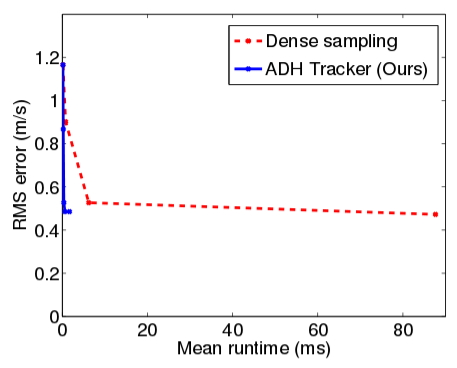
\includegraphics[width=0.6\textwidth]{../img/adh-dense-time}};
    \node (descx) at (7,-0.2)
    {\tiny \cite{paper}};
  \end{tikzpicture}
  \end{itemize}
  \end{description}
\end{frame}

\begin{frame}
  \frametitle{Evaluation}
  \begin{description}[]
  \item[] \hfill \\
  \begin{itemize}
  \item Relative reference frame precise but not realistic
  \end{itemize}
  \pause
  \item[Model Crispness Approach] \hfill \\
  \begin{itemize}
  \item Build a model of the tracked object
  \item Union object point clouds over all frames
  \item Point clouds aligned by position estimation
  \begin{tikzpicture}[thick, every node/.style={font=\footnotesize}]
    \node (program) [outer sep=0,inner sep=0,anchor=south west]
    at (0,0)
    {
    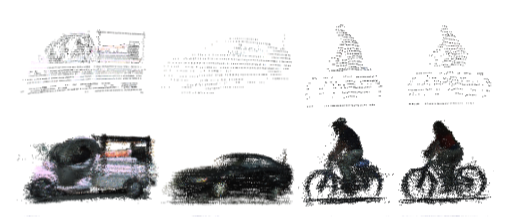
\includegraphics[width=0.6\textwidth]{../img/build-models}};
    \node (descx) at (7,-0.2)
    {\tiny \cite{paper}};
  \end{tikzpicture}
  \item Record sensor data in real traffic
  \onslide<1->
  \end{itemize}
  \end{description}
\end{frame}

\begin{frame}
  \frametitle{Evaluation}
  \begin{description}[]
  \item[Crispness Score] \hfill \\
  \begin{itemize}
  \item Measure for distinctness of the build model
  \pause
  \end{itemize}
  \end{description}
  \begin{columns}
  \begin{column}{0.5\textwidth}
  \center
  \begin{tikzpicture}[thick, every node/.style={font=\footnotesize}]
    \node (program) [outer sep=0,inner sep=0,anchor=south west]
    at (0,0)
    {
    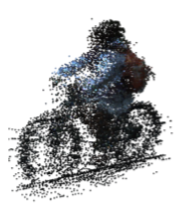
\includegraphics[width=0.5\textwidth,height=0.6\textwidth]{../img/model-adh}};
    \node (descx) at (2.5,-0.2)
    {\tiny \cite{paper}};
  \end{tikzpicture}
  \begin{itemize}
  \item Presented tracker
  \item High crispness score
  \end{itemize}
  \end{column}
  \begin{column}{0.5\textwidth}
  \center
  \begin{tikzpicture}[thick, every node/.style={font=\footnotesize}]
    \node (program) [outer sep=0,inner sep=0,anchor=south west]
    at (0,0)
    {
    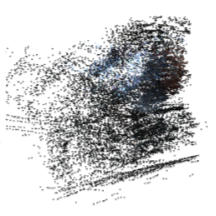
\includegraphics[width=0.5\textwidth,height=0.6\textwidth]{../img/model-icp}};
    \node (descx) at (2.5,-0.2)
    {\tiny \cite{paper}};
  \end{tikzpicture}
  \begin{itemize}
  \item Kalman ICP tracker
  \item Low crispness score
  \end{itemize}
  \end{column}
  \end{columns}
\end{frame}

\begin{frame}
  \frametitle{Evaluation}
  \begin{tikzpicture}[thick, every node/.style={font=\footnotesize}]
    \node (program) [outer sep=0,inner sep=0,anchor=south west]
    at (0,0)
    {
    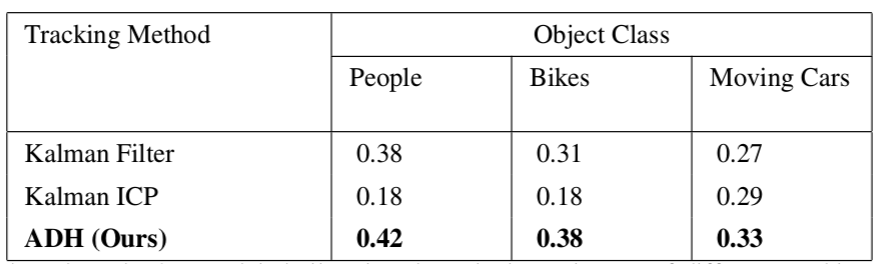
\includegraphics[width=\textwidth]{../img/crispness-scores}};
    \node (descx) at (10,-0.2)
    {\tiny \cite{paper}};
  \end{tikzpicture}
  \begin{itemize}
  \item Highest score for all object classes
  \item Higher score for people than for cars
  \end{itemize}
\end{frame}

\begin{frame}
  \frametitle{Evaluation}
  \begin{description}[]
  \item[Improvement through color model] \hfill \\
  \begin{itemize}
  \item RMS error decreased by $10.4\%$
  \item $p(C)$ very small (lens flare, heavy shadows)
  \item Works robust through day-times and seasons
  \end{itemize}
  %% \item[Align smaller point cloud in larger one] \hfill \\
  %% \begin{itemize}
  %% \item RMS error decreased by $10\%$
  %% \end{itemize}
  \item[Source Code] \hfill \\
  \begin{itemize}
  \item Open Source\\
        \url{http://stanford.edu/~davheld/anytime_tracking.html}
  \item Easy to setup, integrate into C++
  \item Test-data available
  \end{itemize}
  \item[Performance with stereo camera data?] \hfill \\
  \begin{itemize}
  \item Cheaper sensor, more noisy data
  \item A lot of configuration values in the code
  \end{itemize}
  \end{description}
\end{frame}

\section{Conclusion}
\begin{frame}
  \frametitle{Conclusion}       
  \begin{block}{Combine 3D Shape, Color, Motion for Robust Anytime Tracking}
    Precise and robust tracking is possible in real-time
  \end{block}
  \begin{itemize}
  \item Measurement model combines 3D shape, Color, Motion
  \item Derived from Dynamic Bayesian Network
  \item Annealed Dynamic Histogram for global and fast search
  \item Evaluation with local reference frame and model crispness
  \item Outperforms baseline methods
  \end{itemize}
\end{frame}



\backupbegin

\begin{frame}[allowframebreaks]
  \frametitle{References}
  %% \nocite{*}
  \bibliographystyle{splncs}
  \bibliography{references}
\end{frame}

\begin{frame}
  \frametitle{Backup slide}
  \begin{description}[]
  \item[Crispness score formula] \hfill \\
  \begin{itemize}
  \item $$\frac{1}{T^2}\sum_{i=1}^T\sum_{j=1}^T\frac{1}{n_i}\sum_{k=1}^{n_i}G(x_k-\hat{x}_k,2\Sigma)$$
  \end{itemize}
  \end{description}
\end{frame}

\begin{frame}
  \frametitle{Backup slide: RoboCup Logistics League}
  \begin{columns}
  \begin{column}{0.5\textwidth}
  \center
  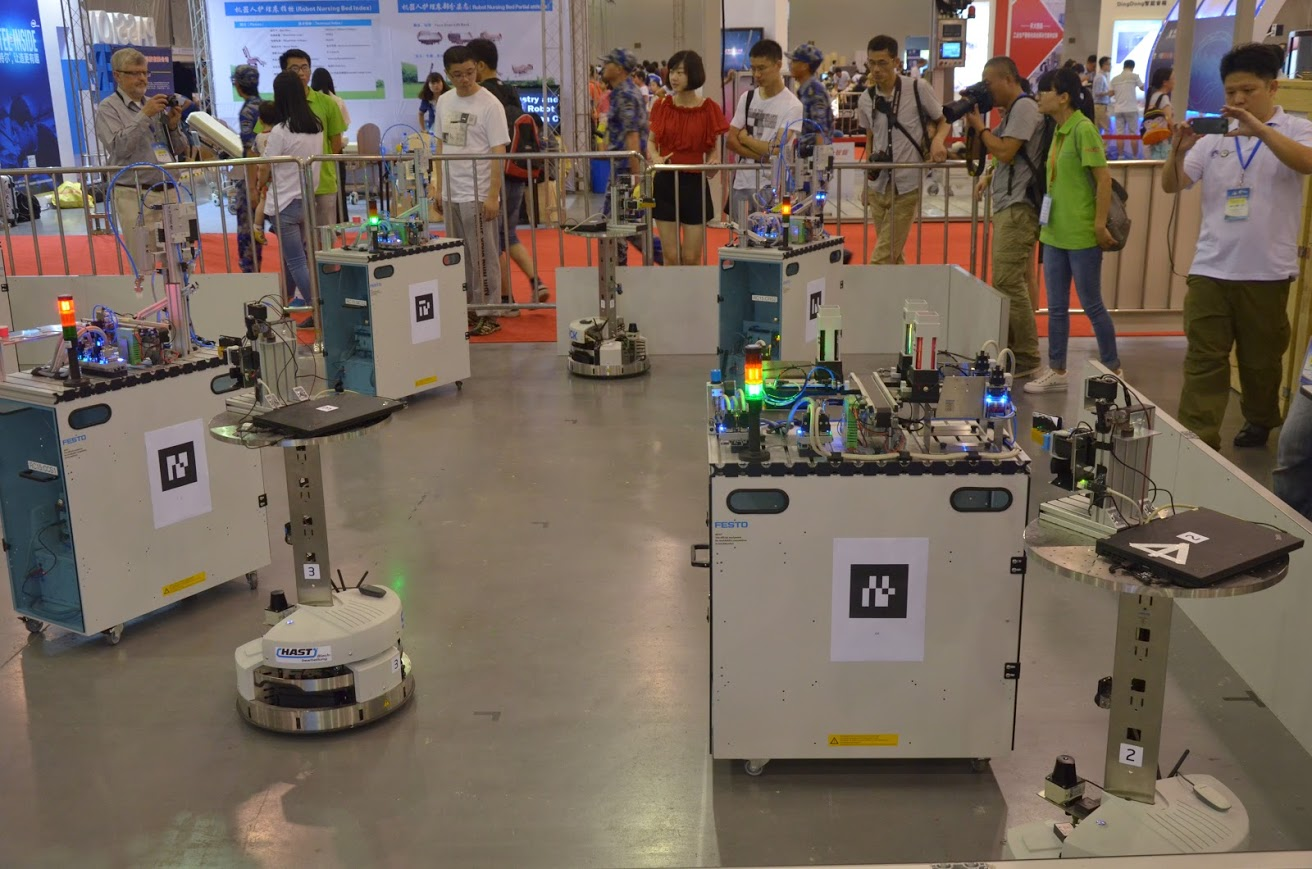
\includegraphics[width=0.9\textwidth]{images/DSC_6148}\\  
  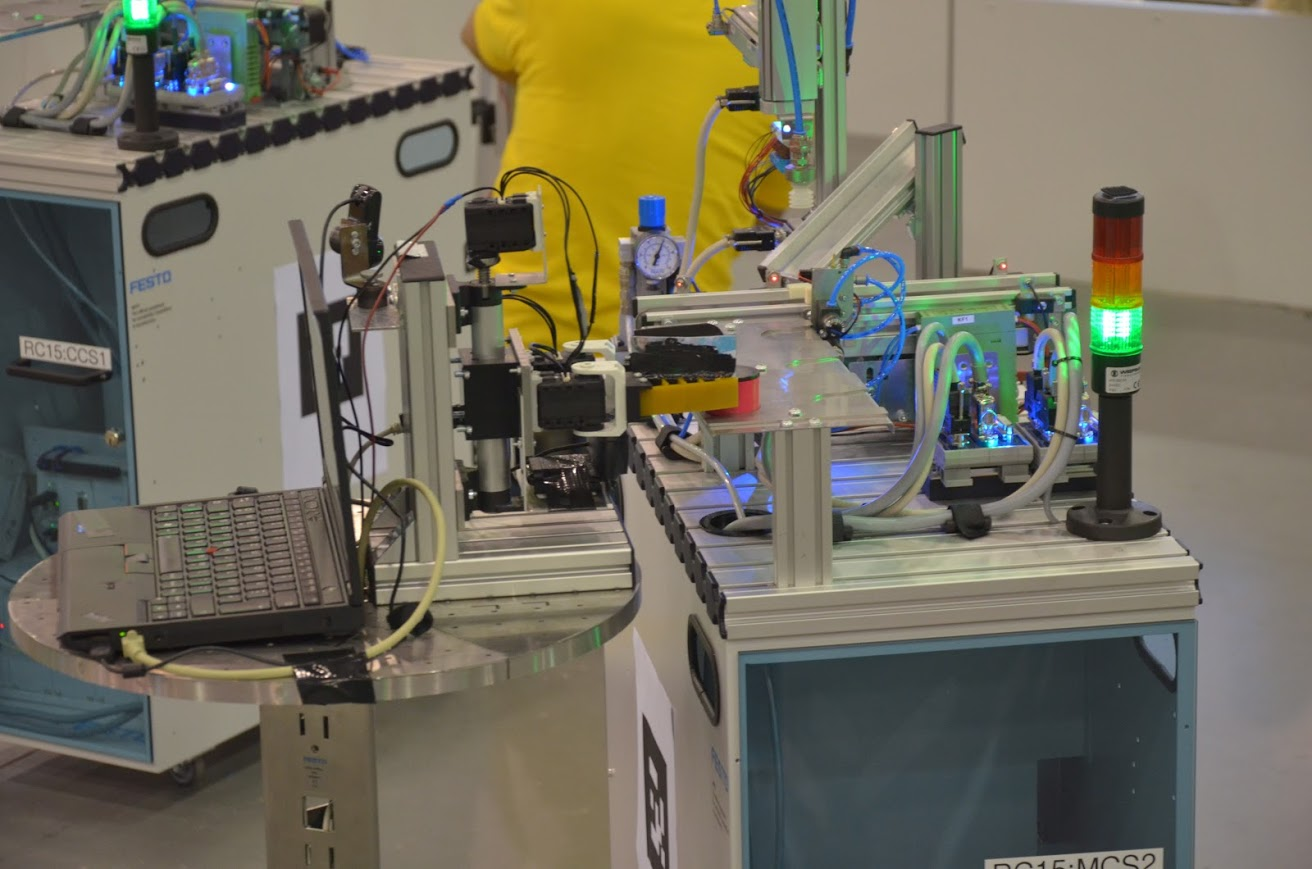
\includegraphics[width=0.9\textwidth]{images/DSC_6497}  
  \end{column}
  \begin{column}{0.5\textwidth}
  \center
  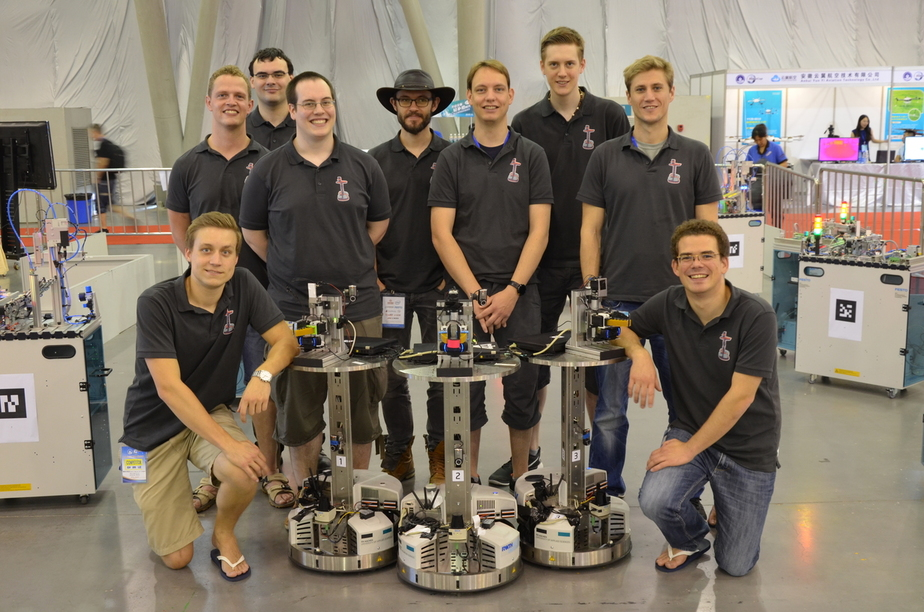
\includegraphics[width=0.9\textwidth]{images/DSC_6846}\\
  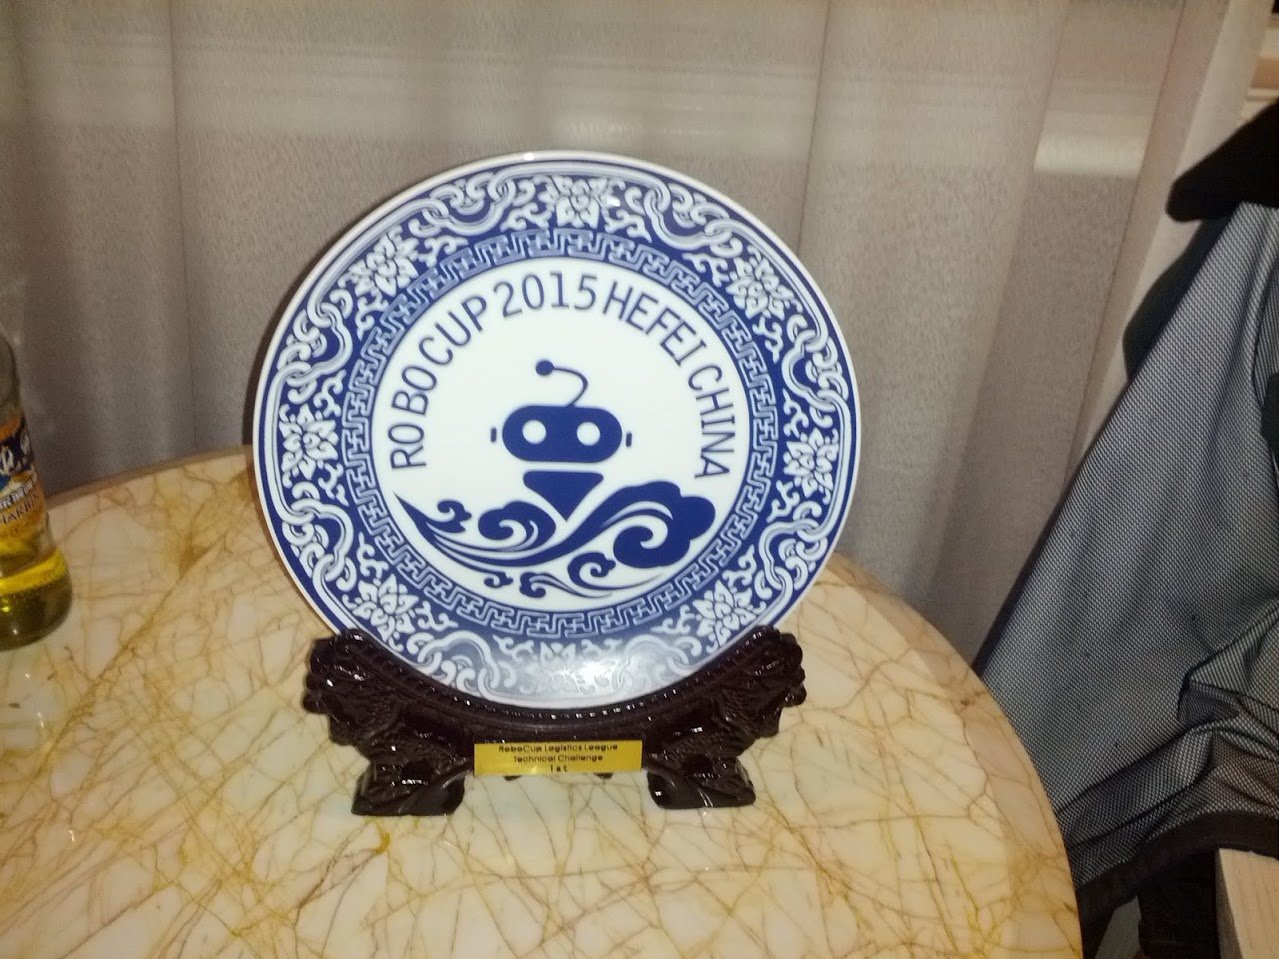
\includegraphics[width=0.9\textwidth]{images/preis}
  \end{column}
  \end{columns}
\end{frame}

\backupend

\end{document}
